\section{Uniform separation from the six central openings}\label{sec:separation}
\subsection{The individual-hull envelope}\label{sec:hulls}
For each of the six boundaries define its individual convex enclosure
\begin{equation}\label{eq:hulls}
 \Hull_k^\sigma=\operatorname{conv}(G_k^\sigma).
\end{equation}
It is the triangle formed by that boundary's elbow and two tips. This is a mathematical bounding set, not a declaration that an opening is a filled material aperture. Each upper hull lies in $h_g\le\zeta\le H_0$; each lower hull lies in $-H_0\le\zeta\le-h_g$.

For any spatial point let $r_\perp(P)=\norm{P_h}$ be its cylindrical radius about the axis through $O$, and set
\begin{equation}\label{eq:separator}
 \Phi(P)=r_\perp(P)-\frac35|\zeta(P)|,\qquad
 D_* =\sqrt{10-6\sqrt2},\qquad L_* =\frac{\sqrt{34}}5.
\end{equation}
Since $J_\perp^T=-J_\perp$ and $J_\perp^TJ_\perp=I$,
\begin{equation}\label{eq:similarity}
 A_{\tau_g}^TA_{\tau_g}
 =\left(1+\frac{\tau_g^2}{r_g^2}\right)I,\qquad
 \sqrt{1+\tau_g^2/r_g^2}\le\sqrt{1+h_g^2/r_g^2}=D_*.
\end{equation}
Every elbow therefore has cylindrical radius at most $D_*a_g$, and every tip at most $D_*r_g$. Reflection preserves both radius and absolute height. The exact vertex inequalities are
\begin{equation}\label{eq:vertexbounds}
 D_*a_g-\frac35h_g<\frac3{50},\qquad
 D_*r_g-\frac35H_0<\frac3{50}.
\end{equation}
Appendix~\ref{sec:arithmetic} gives rational certificates for these comparisons.

\begin{proposition}[Uniform individual-hull envelope]\label{prop:hullenvelope}
For every $k$, sign $\sigma$, admitted $\tau_g$ and hand,
\begin{equation}\label{eq:envelope}
 \Phi(Q)\le\frac3{50}\qquad(Q\in\Hull_k^\sigma).
\end{equation}
\end{proposition}
\begin{proof}
On either fixed-sign height halfspace, $\Phi$ is a norm minus a linear function, hence convex. Each individual hull stays in one such halfspace. Convexity and \eqref{eq:vertexbounds} bound every convex combination of its three vertices. More explicitly, if $t$ is the total weight of the two tips, then
\begin{equation}\label{eq:hullinterpolation}
 |\zeta(Q)|=(1-t)h_g+tH_0,\qquad
 r_\perp(Q)\le D_*[(1-t)a_g+tr_g],\quad 0\le t\le1.
\end{equation}
Subtracting three fifths of the height makes the estimate a convex combination of the two vertex bounds. Both endpoints of the static parameter range are included.
\end{proof}

One cannot replace the six individual hulls by their combined convex hull: $\Phi$ is not globally convex. At $\tau_g=0$, an upper and lower tip at the same horizontal position $r_ge_{2k}$ have midpoint $(r_ge_{2k},0)$, with $\Phi=r_g>3/50$, although each tip has $\Phi=r_g-3/10<3/50$. This is why the fixed-sign condition is essential.

\subsection{The carrier separator and a Euclidean bound}\label{sec:clearance}
Because $K_c/\RG=(2+\sqrt3)/\sqrt7>1$, the coefficient $K_c+\RG\cos\theta$ never changes sign. For every geometric circle,
\begin{equation}\label{eq:cylindrical}
 r_\perp(\Gamma_j(\theta))=K_c+\RG\cos\theta,\qquad
 \zeta(\Gamma_j(\theta))=\RG\sin\theta.
\end{equation}
This cylindrical radius differs from the radial distance $D$ in \eqref{eq:radial}. Cauchy--Schwarz on $(\cos\theta,|\sin\theta|)$ gives
\begin{equation}\label{eq:carriergap}
 \Phi(\Gamma_j(\theta))\ge K_c-L_*\RG,
 \qquad \Delta_*:=K_c-L_*\RG-\frac3{50}>0.
\end{equation}
The strict positivity is certified below. The scalar-function gap is not yet a spatial distance. For arbitrary points, including the axis and opposite height signs, reverse triangle inequalities give
\begin{equation}\label{eq:lipschitz}
 \begin{aligned}
 |\Phi(P)-\Phi(Q)|
 &\le |r_\perp(P)-r_\perp(Q)|+\tfrac35\big||\zeta(P)|-|\zeta(Q)|\big|\\
 &\le\norm{P_h-Q_h}+\tfrac35|\zeta(P)-\zeta(Q)|\\
 &\le L_*\norm{P-Q}.
 \end{aligned}
\end{equation}
This is a global Lipschitz estimate and uses no differentiability at the norm's singular points.

\begin{theorem}[Uniform six-opening clearance]\label{thm:separation}
Under the common geometric scaling of all centered coordinates and the static parameter by $\wh>0$, every geometric circle and every individual hull satisfy, for all admitted $\tau_g$, both hands, all $j,k$ and $\sigma$,
\begin{equation}\label{eq:distance}
 \operatorname{dist}(\Gamma_{j,\wh},\Hull_{k,\wh}^{\sigma,\mathrm{hand}})
 \ge\wh\frac{\Delta_*}{L_*}
 >\frac{23107}{389000}\wh
 >\frac{297}{5000}\wh.
\end{equation}
The same bound holds with the actual broken boundary $G_{k,\wh}^{\sigma,\mathrm{hand}}$ in place of its hull.
\end{theorem}
\begin{proof}
At width one, \eqref{eq:envelope} and \eqref{eq:carriergap} imply $\Phi(P)-\Phi(Q)\ge\Delta_*$ for every circle point $P$ and hull point $Q$. Equation~\eqref{eq:lipschitz} gives $\norm{P-Q}\ge\Delta_*/L_*$. Taking the infimum proves the non-strict estimate. The rational bounds in Appendix~\ref{sec:arithmetic} establish
\begin{equation}\label{eq:coarsegap}
 \Delta_*>\frac{69321}{1000000},\qquad L_*<\frac{1167}{1000},\qquad
 \frac{69321/1000000}{1167/1000}=\frac{23107}{389000}>\frac{297}{5000}.
\end{equation}
All divisions involve positive quantities. The subset $G\subset\Hull$ gives the boundary statement. Common scaling multiplies distances, $r_\perp$, $|\zeta|$ and the gap by $\wh$ while leaving $\tau_g/r_g$ and $L_*$ unchanged.
\end{proof}

The exact conservative expression $\Delta_*/L_*$ is approximately $0.06097180165653555$ at width one. It is not the actual minimum distance or an optimized clearance: saturation of the circle separator does not imply that any hull point saturates its envelope at a closest pair. The rational conclusion in \eqref{eq:distance} is independent of this decimal display.

\begin{figure}[htbp]\centering
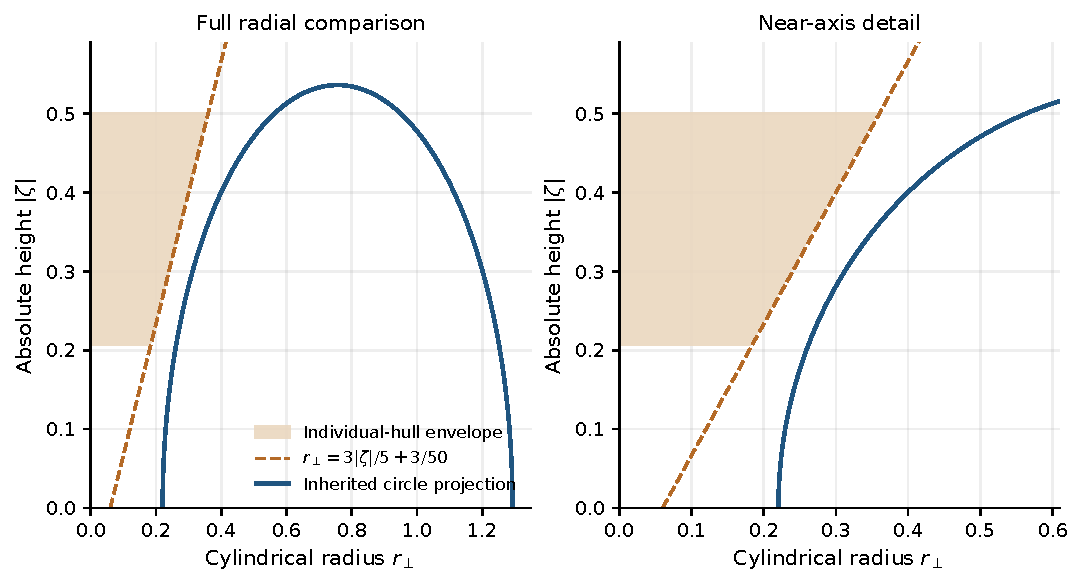
\includegraphics[width=\textwidth]{figures/six_opening.pdf}
\caption{Radial/absolute-height projection at width one: the full comparison (left) and a close view (right). The shading bounds each individual $G$ hull using \eqref{eq:hullinterpolation}; it is not a physical aperture. The dashed separator is $r_\perp=3|\zeta|/5+3/50$. The circle lies strictly on its exterior side for all angles. Rotation and full reflection leave these projected quantities unchanged. Sampled plotting points illustrate the exact inequalities; they do not establish the uniform theorem.}\label{fig:separation}
\end{figure}

\Needspace{9\baselineskip}
\begin{corollary}[No direct crossing parameter]\label{cor:empty}
For every circle in the unchanged registration,
\begin{equation}\label{eq:empty}
 \Gamma_j^{-1}(G_k^{\sigma,\mathrm{hand}})=\varnothing,
 \qquad \Gamma_j^{-1}(\Hull_k^{\sigma,\mathrm{hand}})=\varnothing.
\end{equation}
The spatial images $\gamma_0(S_\pm)$ of the finite source/loading supports obey the same lower distance bound.
\end{corollary}
\begin{proof}
An intersection would have distance zero, contradicting Theorem~\ref{thm:separation}. The support images are subsets of $\Gamma_0$.
\end{proof}

Changing arclength width along this curve cannot create off-curve incidence. The theorem covers a future aperture \emph{if} it lies wholly within its individual hull, but no such aperture has been adopted. An unspecified thick tube, nonplanar spanning surface or relative translation or rescaling of one object requires a separate analysis. The common-width result is geometric and does not assign physical units.
